% Provenance (never printed): cycle 3 / 6e "La planete Terre" (structure of
% the globe: crust, mantle, core); see sources/book1/PROVENANCE.md. Book 1,
% grade 6, chapter 4.
% Vocabulary guard: "magma" not before g7.2 ("molten rock"); P and S waves,
% Moho, core--mantle boundary and lithosphere belong to Book 2 (g11): the
% waves are told in prose, never defined; "seismometer" is defined in g7.3.
\chapter{O interior da Terra}\label{ch:g6:inside-the-earth}

No extremo noroeste da Rússia, não muito longe da fronteira com a Noruega, uma tampa de metal está soldada no chão, no meio de prédios abandonados. Embaixo dela, um buraco de
apenas 23~centímetros de largura desce reto por mais de 12~quilômetros: é o
buraco mais fundo já cavado. Perfurá-lo levou cerca de 20~anos. Os
perfuradores esperavam ir ainda mais fundo, mas, no fundo, a \omterm{def:g3:stones-pebbles-sand:rock}{rocha} estava a
cerca de 180~graus Celsius, quase o dobro do esperado: o calor entortou as
brocas e os tubos, e o trabalho parou em 1992. Mesmo assim, o centro da
Terra fica mais de \textbf{500 vezes} mais fundo que o fundo desse buraco.
Como podemos saber o que existe lá embaixo?
% ledger: sciam:kola-depth, sciam:kola-180C, earth:Rmean

\begin{omfigure}
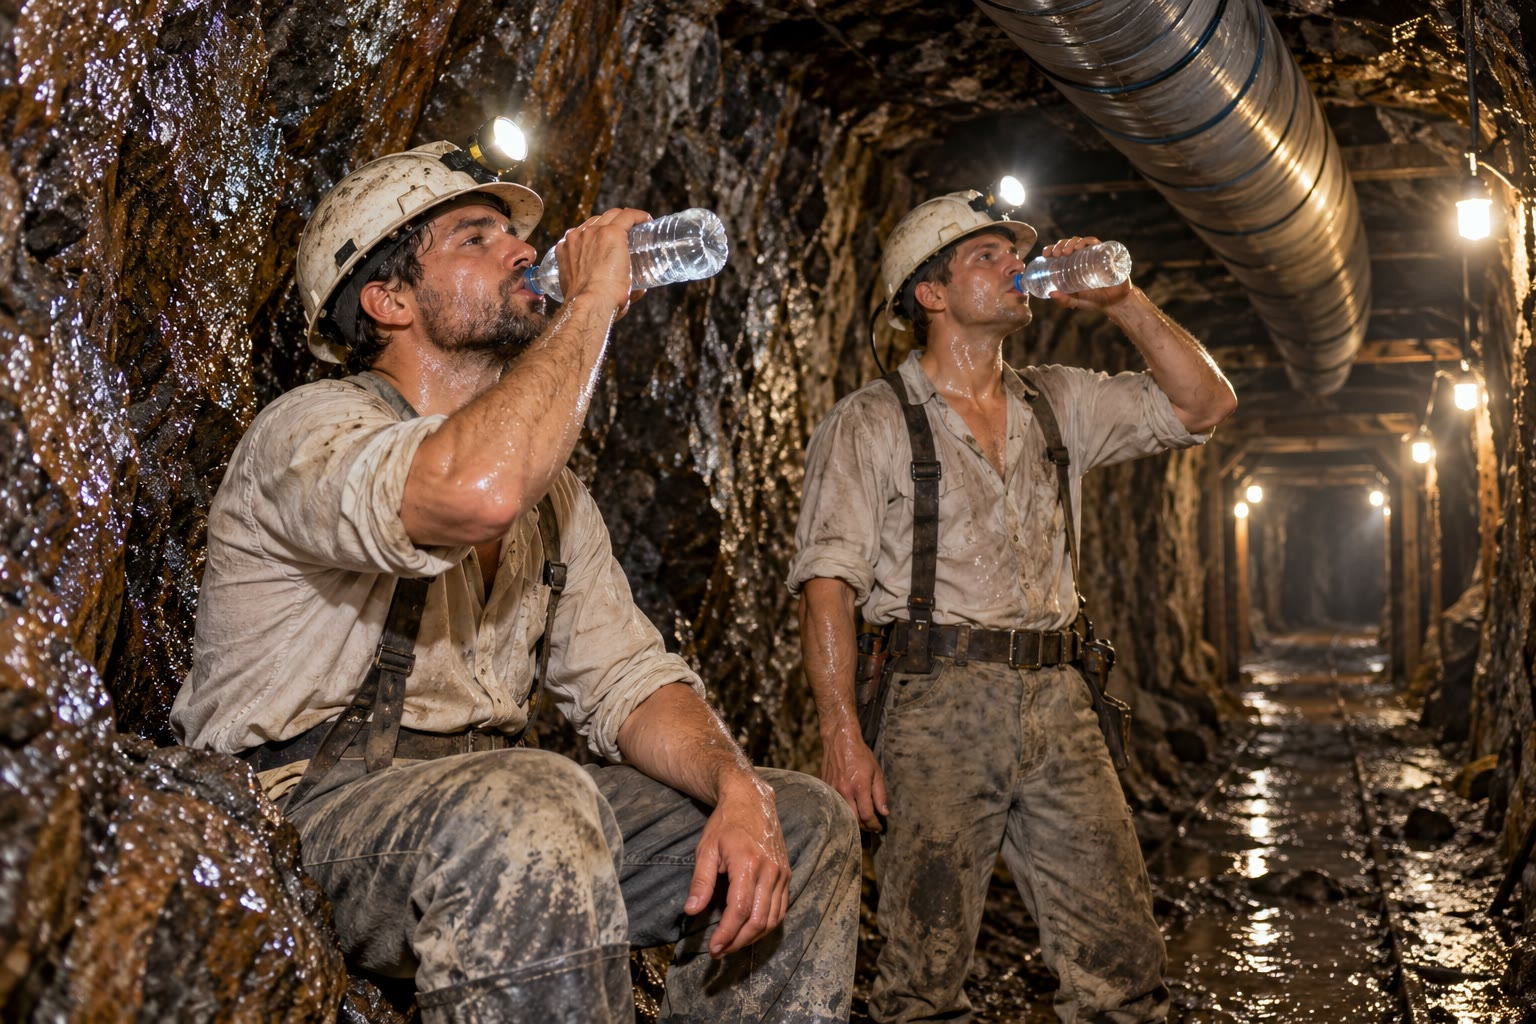
\includegraphics[width=0.62\linewidth]{images/book1/ai/g6-deep-mine.jpg}

{\small Mineiros bebem água numa galeria quente, a quilômetros embaixo da
terra. (Ilustração feita por IA.)}
\end{omfigure}

\begin{recall}
A Terra é um \omterm{def:g6:earth-a-planet:planet-types}{planeta rochoso}, uma bola de cerca de 12\,742~km de diâmetro:
o seu raio, da superfície até o centro, é de cerca de 6371~km
(\cref{ch:g6:earth-a-planet}). As suas \omterm{def:g3:stones-pebbles-sand:rock}{rochas} pertencem a três famílias,
ígneas, sedimentares e metamórficas (\cref{ch:g6:rocks-and-minerals}). Num
\omterm{def:g4:volcanoes-earthquakes-first-look:volcano}{vulcão}, a \omterm{def:g3:stones-pebbles-sand:rock}{rocha} derretida sobe de baixo e se derrama como \omterm{def:g4:volcanoes-earthquakes-first-look:eruption}{lava}; num
\omterm{def:g4:volcanoes-earthquakes-first-look:earthquake}{terremoto}, o chão treme (\cref{ch:g4:volcanoes-earthquakes-first-look}).
\end{recall}
% ledger: earth:Rmean

\section{Até que profundidade já chegamos?}

Há muito tempo as pessoas cavam a Terra, em busca de água, de pedra e de
metais. Dois tipos de buraco são os que vão mais fundo.

\textbf{As minas.} A mina mais funda do mundo é uma mina de ouro perto de
Joanesburgo, na África do Sul. As suas galerias descem mais de 4~km abaixo
da superfície. Lá embaixo, as paredes de \omterm{def:g3:stones-pebbles-sand:rock}{rocha} chegam a cerca de
60~graus Celsius: a mina é resfriada com milhares de toneladas de gelo
misturado com água, bombeadas lá para baixo, e com ventiladores gigantes
que sopram ar pelas galerias.
% ledger: gwr:deepest-mine

\textbf{Os furos de sondagem.} Um furo de sondagem é um buraco estreito
perfurado a partir da superfície por uma máquina; ninguém desce por ele. O
mais fundo é o furo da história do começo, cavado para a ciência na
península de Kola, no noroeste da Rússia: 12\,262~metros, ou seja, cerca de
12.3~km.
% ledger: sciam:kola-depth

Essas profundidades parecem enormes. Comparadas com o tamanho da Terra,
elas são minúsculas. A figura abaixo as mostra numa só faixa, ao lado da
\omterm{def:g1:landscapes-around-us:landform}{montanha} mais alta, o monte Everest (8849~m).
% ledger: tht:everest

\begin{omfigure}
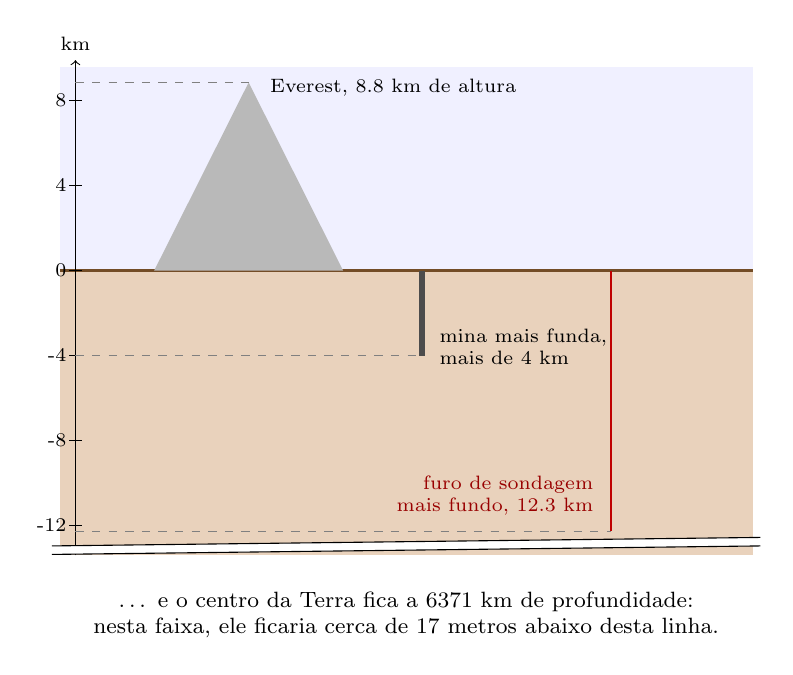
\begin{tikzpicture}[yscale=0.27, xscale=1]
  % sea-level ground and the sky
  \fill[blue!6] (-0.2,0) rectangle (8.6,9.6);
  \fill[brown!35] (-0.2,0) rectangle (8.6,-13.4);
  \draw[thick, brown!60!black] (-0.2,0) -- (8.6,0);
  % depth axis
  \draw[->] (0,-13.4) -- (0,9.9) node[above, font=\scriptsize] {km};
  \foreach \y in {-12,-8,-4,0,4,8} \draw (-0.08,\y) -- (0.08,\y) node[left=2pt, font=\scriptsize] {\y};
  % Everest
  \fill[gray!55] (1.0,0) -- (2.2,8.849) -- (3.4,0) -- cycle;
  \draw[dashed, gray] (0,8.849) -- (2.2,8.849);
  \node[font=\scriptsize, right] at (2.35,8.6) {Everest, 8.8~km de altura};
  % deepest mine
  \draw[line width=2.2pt, black!70] (4.4,0) -- (4.4,-4);
  \draw[dashed, gray] (0,-4) -- (4.4,-4);
  \node[font=\scriptsize, right, align=left] at (4.5,-3.6) {mina mais funda,\\ mais de 4~km};
  % Kola borehole
  \draw[line width=0.7pt, red!75!black] (6.8,0) -- (6.8,-12.262);
  \draw[dashed, gray] (0,-12.262) -- (6.8,-12.262);
  \node[font=\scriptsize, left, align=right, red!60!black] at (6.7,-10.6) {furo de sondagem\\ mais fundo, 12.3~km};
  % break and the centre
  \draw[white, line width=3pt] (-0.3,-13.15) -- (8.7,-12.75);
  \draw (-0.3,-13.35) -- (8.7,-12.95);
  \draw (-0.3,-12.95) -- (8.7,-12.55);
  \node[font=\footnotesize, align=center] at (4.2,-16.2) {\ldots\ e o centro da Terra fica a 6371~km de profundidade:\\
     nesta faixa, ele ficaria cerca de 17~metros abaixo desta linha.};
\end{tikzpicture}

{\small Alturas e profundidades desenhadas na mesma escala (1~cm para
3.7~km), a partir do \omterm{def:g4:world-physical-map:altitude}{nível do mar}. A interrupção na faixa esconde quase
todo o caminho até o centro.}
% ledger: tht:everest, gwr:deepest-mine, sciam:kola-depth, earth:Rmean
\end{omfigure}

\begin{method}[Comparar uma profundidade com o raio da Terra]\label{met:g6:inside-the-earth:percent}
\begin{enumerate}
  \item Escreva a profundidade e o raio na mesma unidade (quilômetros).
  \item Divida a profundidade pelo raio e depois multiplique por 100: isso
        dá a profundidade como porcentagem do caminho até o centro.
  \item Para dizer quantas vezes o centro é mais fundo, divida o raio pela
        profundidade.
\end{enumerate}
\end{method}

\begin{example}[O furo de sondagem mais fundo]\label{ex:g6:inside-the-earth:kola}
O furo tem 12.3~km de profundidade, e o raio é de 6371~km.
$12.3 \div 6371 \approx 0.0019$, e $0.0019 \times 100 = 0.19$: o furo
percorreu cerca de \textbf{0.2~\%} do caminho até o centro. No sentido
contrário, $6371 \div 12.3 \approx 518$: o centro fica mais de 500~vezes
mais fundo que o fundo do buraco.

Para a mina mais funda, cerca de 4~km: $4 \div 6371 \approx 0.0006$, ou
seja, 0.06~\%: três vezes menos que o furo.
% ledger: sciam:kola-depth, earth:Rmean, gwr:deepest-mine
\end{example}

Então ninguém nunca viu, tocou ou recolheu amostras do interior profundo
da Terra. O que sabemos dele vem de outras pistas, sobretudo das ondas dos
\omterm{def:g4:volcanoes-earthquakes-first-look:earthquake}{terremotos} (seção~\ref{sec:g6:inside-the-earth:waves}).

\section{Crosta, manto e núcleo}

A Terra é construída em camadas, um pouco como um ovo cozido: uma casca
fina e quebradiça, uma ``clara'' grossa e uma ``gema'' no meio.
% ledger: usgs:layers-egg

\begin{omfigure}
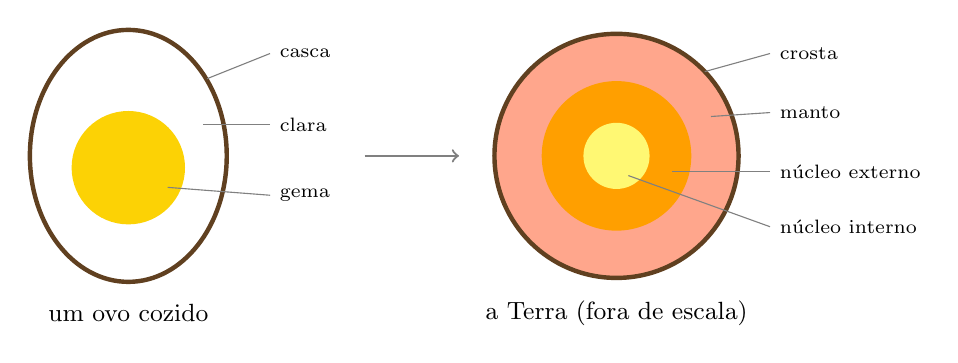
\begin{tikzpicture}
  % a boiled egg cut in half
  \begin{scope}
    \fill[white] (0,0) ellipse (1.25 and 1.6);
    \draw[brown!50!black, line width=1.6pt] (0,0) ellipse (1.25 and 1.6);
    \fill[yellow!70!orange] (0,-0.15) circle (0.72);
    \node[font=\scriptsize, anchor=west] (s) at (1.8,1.3) {casca};
    \draw[gray] (s.west) -- (1.0,0.98);
    \node[font=\scriptsize, anchor=west] (w) at (1.8,0.4) {clara};
    \draw[gray] (w.west) -- (0.95,0.4);
    \node[font=\scriptsize, anchor=west] (y) at (1.8,-0.5) {gema};
    \draw[gray] (y.west) -- (0.5,-0.4);
    \node[font=\small] at (0,-2.0) {um ovo cozido};
  \end{scope}
  \draw[->, thick, gray] (3.0,0) -- (4.2,0);
  % the Earth, not to scale
  \begin{scope}[xshift=6.2cm]
    \fill[orange!45!red!45] (0,0) circle (1.55);
    \fill[orange!75!yellow] (0,0) circle (0.95);
    \fill[yellow!55] (0,0) circle (0.42);
    \draw[brown!50!black, line width=1.6pt] (0,0) circle (1.55);
    \node[font=\scriptsize, anchor=west] (c) at (1.95,1.3) {crosta};
    \draw[gray] (c.west) -- (1.12,1.07);
    \node[font=\scriptsize, anchor=west] (m) at (1.95,0.55) {manto};
    \draw[gray] (m.west) -- (1.2,0.5);
    \node[font=\scriptsize, anchor=west] (o) at (1.95,-0.2) {núcleo externo};
    \draw[gray] (o.west) -- (0.7,-0.2);
    \node[font=\scriptsize, anchor=west] (i) at (1.95,-0.9) {núcleo interno};
    \draw[gray] (i.west) -- (0.15,-0.25);
    \node[font=\small] at (0,-2.0) {a Terra (fora de escala)};
  \end{scope}
\end{tikzpicture}

{\small A Terra comparada com um ovo cozido. Ao contrário da gema, o \omterm{def:g6:inside-the-earth:layers}{núcleo}
tem duas partes. Neste desenho, a \omterm{def:g6:inside-the-earth:layers}{crosta} aparece grossa demais; o desenho
em escala vem logo depois.}
% ledger: usgs:layers-egg
\end{omfigure}

\begin{definition}[As camadas da Terra]\label{def:g6:inside-the-earth:layers}
A Terra é feita de três camadas principais, da superfície até o centro:
\begin{itemize}
  \item a \emph{crosta}\index{crosta}, uma camada externa fina de \omterm{def:g3:stones-pebbles-sand:rock}{rocha}
        sólida, com alguns quilômetros a algumas dezenas de quilômetros de
        espessura;
  \item o \emph{manto}\index{manto}, uma camada grossa de \omterm{def:g3:stones-pebbles-sand:rock}{rocha} sólida,
        quente e densa, até uma profundidade de cerca de 2900~km;
  \item o \emph{núcleo}\index{nucleo@núcleo}, feito de metal, sobretudo ferro com
        um pouco de níquel, de cerca de 2900~km de profundidade até o
        centro. O núcleo tem duas partes: o \emph{núcleo externo}\index{nucleo externo@núcleo externo},
        que é líquido, e o \emph{núcleo interno}\index{nucleo interno@núcleo interno}, uma
        bola sólida no centro, com cerca de 1220~km de raio.
\end{itemize}
% ledger: usgs:layers-egg, usgs:crust-thickness, data:prem, earth:Rmean
\end{definition}

O desenho abaixo mostra as camadas \emph{em escala}, com os limites
medidos pelas ondas dos \omterm{def:g4:volcanoes-earthquakes-first-look:earthquake}{terremotos}.

\begin{omfigure}
\pgfplotstableread{figdata/out/grade-6-earth_layers-disc.dat}\disctab
\pgfplotstablegetelem{0}{r_cm}\of\disctab \let\rE\pgfplotsretval
\pgfplotstablegetelem{1}{r_cm}\of\disctab \let\rOC\pgfplotsretval
\pgfplotstablegetelem{2}{r_cm}\of\disctab \let\rIC\pgfplotsretval
\begin{minipage}[c]{0.43\linewidth}\centering
\begin{tikzpicture}
  \fill[orange!45!red!45] (0,0) circle (\rE cm);
  \fill[orange!75!yellow] (0,0) circle (\rOC cm);
  \fill[yellow!55] (0,0) circle (\rIC cm);
  \draw[brown!50!black, line width=0.45pt] (0,0) circle (\rE cm);
  
  \draw[gray, thin] (-0.25,\rE) rectangle (0.25,\rE-0.12);
  
  \node[font=\scriptsize, align=center, inner sep=0pt] at (0,0) {núcleo\\ interno};
  \node[font=\scriptsize, align=center] at (0,1.03) {núcleo\\ externo};
  \node[font=\scriptsize] at (0,2.12) {manto};
  \draw[<-, font=\scriptsize] (1.98,1.98) -- (2.3,2.75) node[above, align=center] {crosta\\ (um fio de cabelo)};
\end{tikzpicture}
\end{minipage}\hfill
\begin{minipage}[c]{0.55\linewidth}\centering
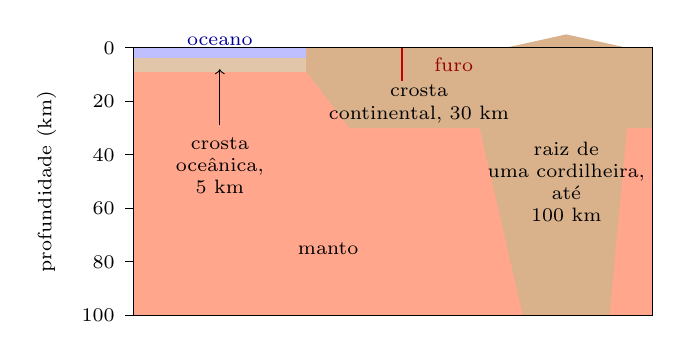
\begin{tikzpicture}[yscale=0.034, xscale=0.55]
  % the top 100 km enlarged: ocean on the left, continent and a range on the right
  \fill[orange!45!red!45] (0,0) rectangle (12,-100);
  \fill[blue!25] (0,0) rectangle (4,-4);
  \fill[brown!45] (0,-4) rectangle (4,-9);                 % oceanic crust 5 km
  \fill[brown!60] (4,0) -- (4,-9) -- (5,-30) -- (8,-30) -- (9,-100) -- (11,-100) -- (11.4,-30) -- (12,-30) -- (12,0) -- cycle;
  \fill[brown!60] (8.6,0) -- (10,5) -- (11.4,0) -- cycle;   % the range (not to scale above ground)
  \draw[red!75!black, line width=0.8pt] (6.2,0) -- (6.2,-12.262);
  \draw[thin] (0,0) rectangle (12,-100);
  \foreach \y in {0,-20,-40,-60,-80,-100} \draw (0,\y) -- (-0.2,\y) node[left, font=\scriptsize] {\pgfmathparse{-\y}\pgfmathprintnumber{\pgfmathresult}};
  \node[font=\scriptsize, rotate=90] at (-2.0,-50) {profundidade (km)};
  \node[font=\scriptsize, align=center] at (2,-44) {crosta\\ oceânica,\\ 5~km};
  \draw[->, thin] (2,-29) -- (2,-8);
  \node[font=\scriptsize, align=center] at (6.6,-21) {crosta\\ continental, 30~km};
  \node[font=\scriptsize, align=center] at (10.0,-50) {raiz de\\ uma cordilheira,\\ até\\ 100~km};
  \node[font=\scriptsize, align=center, red!60!black] at (7.4,-6.5) {furo};
  \node[font=\scriptsize] at (4.5,-75) {manto};
  \node[font=\scriptsize, blue!60!black] at (2,2.5) {oceano};
\end{tikzpicture}
\end{minipage}

\smallskip
{\small À esquerda: a Terra aberta, em escala; o pequeno retângulo cinza no
alto marca a parte ampliada à direita. À direita: os 100~km de cima,
ampliados cerca de 60~vezes: \omterm{def:g6:inside-the-earth:layers}{crosta} fina embaixo dos \omterm{def:g2:water-on-earth:ocean}{oceanos}, mais grossa
embaixo dos \omterm{def:g3:continents-and-oceans:continent}{continentes}, mais grossa ainda embaixo das \omterm{def:g4:world-physical-map:range}{cordilheiras} altas;
o furo recorde em vermelho.}
% ledger: data:prem, earth:Rmean, usgs:crust-thickness, sciam:kola-depth (figdata/grade-6/earth_layers.py)
\end{omfigure}

\begin{center}\small
\begin{tabular}{|l|c|c|c|l|}
\hline
\textbf{camada} & \textbf{de (km)} & \textbf{até (km)} & \textbf{espessura (km)} & \textbf{feita de} \\
\hline
\omterm{def:g6:inside-the-earth:layers}{crosta} & 0 & 5 a 100 & 5 a 100 & \omterm{def:g3:stones-pebbles-sand:rock}{rocha} sólida \\
\omterm{def:g6:inside-the-earth:layers}{manto} & base da \omterm{def:g6:inside-the-earth:layers}{crosta} & 2891 & cerca de 2860 & \omterm{def:g3:stones-pebbles-sand:rock}{rocha} sólida, muito quente \\
\omterm{def:g6:inside-the-earth:layers}{núcleo externo} & 2891 & 5150 & cerca de 2260 & metal líquido \\
\omterm{def:g6:inside-the-earth:layers}{núcleo interno} & 5150 & 6371 (centro) & cerca de 1220 & metal sólido \\
\hline
\end{tabular}
\end{center}
% ledger: data:prem, usgs:crust-thickness, usgs:layers-egg, earth:Rmean (figdata/grade-6/earth_layers.py, main table)

\textbf{A \omterm{def:g6:inside-the-earth:layers}{crosta}} é a única camada em que podemos andar e cavar. Ela é
muito fina comparada com as outras: embaixo dos \omterm{def:g2:water-on-earth:ocean}{oceanos}, ela tem só cerca
de 5~km de espessura; embaixo dos \omterm{def:g3:continents-and-oceans:continent}{continentes}, cerca de 30~km em média;
embaixo de \omterm{def:g4:world-physical-map:range}{cordilheiras} altas como os Alpes, a sua base pode chegar a
100~km de profundidade, como a raiz de um dente. Nem o furo recorde, com 12.3~km de profundidade, atravessou metade de uma \omterm{def:g6:inside-the-earth:layers}{crosta} continental média. No desenho em escala, a \omterm{def:g6:inside-the-earth:layers}{crosta}
é mais fina que a linha em volta do disco.
% ledger: usgs:crust-thickness, sciam:kola-depth

\textbf{O \omterm{def:g6:inside-the-earth:layers}{manto}} é a camada mais grossa: ele vai da base da \omterm{def:g6:inside-the-earth:layers}{crosta} até
2891~km, cerca de 45~\% do caminho até o centro. A sua \omterm{def:g3:stones-pebbles-sand:rock}{rocha} é sólida, mas
muito quente e mais densa que a \omterm{def:g3:stones-pebbles-sand:rock}{rocha} da \omterm{def:g6:inside-the-earth:layers}{crosta}. Ao longo de milhões de
anos, a \omterm{def:g3:stones-pebbles-sand:rock}{rocha} quente de uma parte do \omterm{def:g6:inside-the-earth:layers}{manto} pode se deslocar muito devagar,
como uma pasta muito dura.
% ledger: data:prem, usgs:layers-egg, usgs:lithosphere-80km

\textbf{O \omterm{def:g6:inside-the-earth:layers}{núcleo}} começa a 2891~km e desce até o centro. Ele não é feito de
\omterm{def:g3:stones-pebbles-sand:rock}{rocha}, mas de metal: uma liga de ferro e de níquel, quase duas vezes mais
densa que o \omterm{def:g6:inside-the-earth:layers}{manto}. A sua parte externa é \emph{líquida}: um \omterm{def:g2:water-on-earth:ocean}{oceano} de metal
derretido com mais de 2000~km de profundidade. A sua parte interna, de
5150~km até o centro, é uma bola \emph{sólida} de metal, com cerca de 1220~km de raio: cerca de 70~\% da largura da Lua. Enquanto a Terra gira, o metal líquido do
\omterm{def:g6:inside-the-earth:layers}{núcleo externo} se move, e esse movimento produz o campo magnético da Terra,
o que faz girar a agulha de uma bússola.
% ledger: data:prem, usgs:layers-egg, earth:Rmean, planet:Moon.diameter

Quanto mais fundo, mais denso. A água tem uma densidade de 1~grama por
centímetro cúbico: a \omterm{def:g3:stones-pebbles-sand:rock}{rocha} da \omterm{def:g6:inside-the-earth:layers}{crosta} é de 2.6 a 2.9 vezes mais densa, a
\omterm{def:g3:stones-pebbles-sand:rock}{rocha} da base do \omterm{def:g6:inside-the-earth:layers}{manto} mais de 5~vezes, e o metal do centro cerca de
13~vezes (veja o gráfico abaixo). Os materiais mais pesados ficam no centro e os mais leves em cima: a Terra está organizada, da \omterm{def:g6:inside-the-earth:layers}{crosta} leve até o \omterm{def:g6:inside-the-earth:layers}{núcleo} pesado de metal.
% ledger: data:prem


\begin{omfigure}
\begin{tikzpicture}
  \begin{axis}[omrecord, width=0.86\linewidth, height=5.4cm,
      xmin=0, xmax=6371, ymin=0, ymax=14,
      xlabel={profundidade abaixo da superfície (km)},
      ylabel={densidade (g por cm$^3$)},
      xtick={0,1000,2000,3000,4000,5000,6000},
      scaled x ticks=false, x tick label style={/pgf/number format/1000 sep={}},
      clip=false]
    \fill[orange!45!red!20] (axis cs:24.4,0) rectangle (axis cs:2891,14);
    \fill[orange!75!yellow!35] (axis cs:2891,0) rectangle (axis cs:5149.5,14);
    \fill[yellow!30] (axis cs:5149.5,0) rectangle (axis cs:6371,14);
    \addplot[very thick, black] table[x=depth_km, y=rho] {figdata/out/grade-6-earth_layers-profile.dat};
    \node[font=\scriptsize] at (axis cs:1450,12.5) {manto};
    \node[font=\scriptsize] at (axis cs:4020,4.5) {núcleo externo};
    \node[font=\scriptsize] at (axis cs:5760,4.5) {núcleo interno};
    \node[font=\scriptsize, align=left, anchor=west] at (axis cs:80,1.4) {crosta: de 2.6 a 2.9};
  \end{axis}
\end{tikzpicture}

{\small A densidade da Terra em cada profundidade, segundo um modelo de
referência construído a partir de medições de \omterm{def:g4:volcanoes-earthquakes-first-look:earthquake}{terremotos}. A densidade salta
de cerca de 5.6 para cerca de 9.9~g por cm$^3$ onde a \omterm{def:g3:stones-pebbles-sand:rock}{rocha} do \omterm{def:g6:inside-the-earth:layers}{manto} dá
lugar ao metal do \omterm{def:g6:inside-the-earth:layers}{núcleo}.}
% ledger: data:prem (figdata/grade-6/earth_layers.py, part profile)
\end{omfigure}

\begin{inthelab}[Camadas num copo (em aula, com a professora)]
A professora despeja, devagar e um depois do outro, num copo alto: um
pouco de mel, um pouco de água colorida com uma gota de tinta e um pouco
de óleo de cozinha. Qualquer que seja a ordem, depois de um momento o mel
fica no fundo, a água no meio e o óleo em cima: cada líquido se acomoda
embaixo dos mais leves e em cima dos mais densos. Sacudido, o copo fica
turvo; deixado em paz, ele se organiza de novo. A Terra tem camadas do mesmo jeito: o material mais denso, o metal do \omterm{def:g6:inside-the-earth:layers}{núcleo}, fica no centro, e a \omterm{def:g3:stones-pebbles-sand:rock}{rocha} mais leve fica em cima.
\end{inthelab}


\begin{remark}[Quão fina é a crosta?]\label{rem:g6:inside-the-earth:thin-crust}
Num \omterm{def:g3:continents-and-oceans:globe}{globo} escolar de 30~cm de diâmetro, a \omterm{def:g6:inside-the-earth:layers}{crosta} continental (30~km) teria
cerca de 0.7~milímetro de espessura, e a \omterm{def:g6:inside-the-earth:layers}{crosta} oceânica (5~km), mais ou
menos a espessura de uma folha de papel. A \omterm{def:g6:inside-the-earth:layers}{crosta} tem menos de meio por
cento do raio: $30 \div 6371 \approx 0.0047$, ou seja, 0.47~\%.
% ledger: usgs:crust-thickness, earth:Rmean
\end{remark}

\section{Como as ondas dos terremotos nos contam o resto}\label{sec:g6:inside-the-earth:waves}

Se ninguém foi além de 12~km de profundidade, como podemos desenhar o
\omterm{def:g6:inside-the-earth:layers}{núcleo}? A resposta vem dos \omterm{def:g4:volcanoes-earthquakes-first-look:earthquake}{terremotos}. Quando um \omterm{def:g4:volcanoes-earthquakes-first-look:earthquake}{terremoto} sacode o chão,
ondas partem dele em todas as direções e viajam \emph{através} da Terra
inteira, como o som de uma batida viaja através de uma parede. Instrumentos em muitos lugares do mundo registram quando cada onda chega (você vai conhecê-los no
\cref{ch:g7:earthquakes}).
% ledger: data:prem

As ondas não viajam com a mesma velocidade em todos os materiais. Quando
elas chegam ao limite entre duas camadas, a sua velocidade muda de
repente: algumas ondas voltam, outras se desviam ao atravessar, um pouco
como a luz que entra na água. Medindo o tempo das ondas de muitos \omterm{def:g4:volcanoes-earthquakes-first-look:earthquake}{terremotos}, em estações espalhadas pelo \omterm{def:g3:continents-and-oceans:globe}{globo}, os cientistas descobriram onde ficam esses limites, e
quais camadas são sólidas ou líquidas. Os sismólogos chamam os dois tipos
principais de ondas de \emph{ondas P} (as mais rápidas, que empurram e
puxam a \omterm{def:g3:stones-pebbles-sand:rock}{rocha}) e \emph{ondas S} (as mais lentas, que a sacodem de um lado
para o outro); os volumes seguintes as estudam de perto. As ondas S têm uma
propriedade notável: elas não conseguem atravessar um líquido.

\begin{omfigure}
\begin{tikzpicture}
  \begin{axis}[omrecord, width=0.86\linewidth, height=5.4cm,
      xmin=0, xmax=6371, ymin=0, ymax=14.5,
      xlabel={profundidade abaixo da superfície (km)},
      ylabel={velocidade da onda (km por segundo)},
      xtick={0,1000,2000,3000,4000,5000,6000},
      scaled x ticks=false, x tick label style={/pgf/number format/1000 sep={}},
      clip=false]
    \fill[orange!45!red!20] (axis cs:24.4,0) rectangle (axis cs:2891,14.5);
    \fill[orange!75!yellow!35] (axis cs:2891,0) rectangle (axis cs:5149.5,14.5);
    \fill[yellow!30] (axis cs:5149.5,0) rectangle (axis cs:6371,14.5);
    \addplot[very thick, blue!70!black] table[x=depth_km, y=vp] {figdata/out/grade-6-earth_layers-profile.dat};
    \addplot[very thick, red!75!black] table[x=depth_km, y=vs] {figdata/out/grade-6-earth_layers-profile.dat};
    \node[font=\scriptsize, blue!70!black, anchor=south] at (axis cs:1300,12.9) {ondas P (mais rápidas)};
    \node[font=\scriptsize, red!75!black, anchor=north] at (axis cs:1500,6.1) {ondas S (mais lentas)};
    \node[font=\scriptsize, red!75!black, align=center, fill=white, fill opacity=0.8, text opacity=1] at (axis cs:4020,1.9) {ondas S: 0\\ (líquido)};
    \node[font=\scriptsize] at (axis cs:4020,13.6) {núcleo externo};
    \node[font=\scriptsize] at (axis cs:5760,13.6) {núcleo interno};
    \node[font=\scriptsize] at (axis cs:1450,1.5) {manto};
  \end{axis}
\end{tikzpicture}

{\small A velocidade dos dois tipos de ondas dos \omterm{def:g4:volcanoes-earthquakes-first-look:earthquake}{terremotos} em cada
profundidade, no mesmo modelo de referência. No \omterm{def:g6:inside-the-earth:layers}{núcleo externo}, as ondas S
param: a sua velocidade é zero, porque o \omterm{def:g6:inside-the-earth:layers}{núcleo externo} é líquido.}
% ledger: data:prem (figdata/grade-6/earth_layers.py, part profile)
\end{omfigure}

Lendo o gráfico da esquerda para a direita: no \omterm{def:g6:inside-the-earth:layers}{manto}, os dois tipos de
ondas ficam cada vez mais rápidos com a profundidade. A 2891~km, as ondas S
desaparecem e as ondas P ficam mais lentas de repente: é o topo do \omterm{def:g6:inside-the-earth:layers}{núcleo
externo} líquido. A 5150~km, as ondas P aceleram de novo e as ondas S voltam
a existir: é o \omterm{def:g6:inside-the-earth:layers}{núcleo interno} sólido.
% ledger: data:prem

\begin{history}[Inge Lehmann e o núcleo interno]
\begin{minipage}[c]{0.72\linewidth}
No começo dos anos 1930, os sismólogos achavam que a Terra tinha duas camadas: um \omterm{def:g6:inside-the-earth:layers}{manto} sólido em volta de um \omterm{def:g6:inside-the-earth:layers}{núcleo} líquido. A sismóloga dinamarquesa Inge Lehmann estudou as ondas de
um forte \omterm{def:g4:volcanoes-earthquakes-first-look:earthquake}{terremoto} que atingiu a Nova Zelândia em 1929, registradas em
estações muito distantes. Algumas ondas chegavam a lugares onde, com um
\omterm{def:g6:inside-the-earth:layers}{núcleo} todo líquido, elas não deveriam chegar. Num artigo de 1936, chamado
simplesmente ``P\,$'$'', ela propôs uma explicação: dentro do \omterm{def:g6:inside-the-earth:layers}{núcleo}
líquido existe um \emph{\omterm{def:g6:inside-the-earth:layers}{núcleo interno} sólido} menor, que manda essas ondas
de volta. Ela escreveu com modéstia que os dados eram ``bastante
insuficientes'' para ter certeza, mas que a interpretação ``parece
possível'', e pediu a outros pesquisadores que a testassem. Eles testaram, e hoje o \omterm{def:g6:inside-the-earth:layers}{núcleo interno} sólido faz parte de todos os modelos de referência da Terra, como o que foi usado nos gráficos deste capítulo.
% ledger: nbi:lehmann-1936
\end{minipage}\hfill
\begin{minipage}[c]{0.24\linewidth}\centering
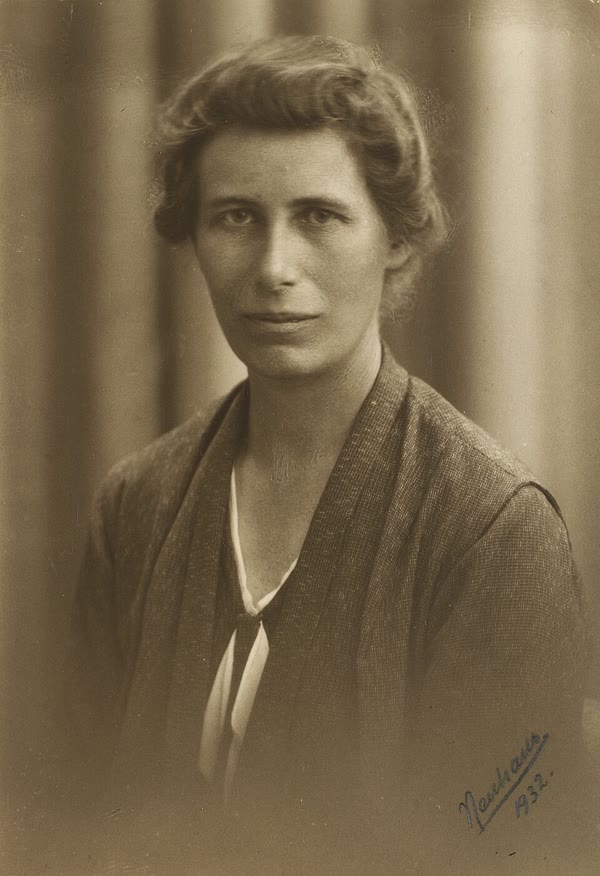
\includegraphics[width=\linewidth]{images/book1/g6-inge-lehmann.jpg}\\[2pt]
{\footnotesize Inge Lehmann em 1932. (Foto: Even Neuhaus, domínio
público, via Wikimedia Commons.)}
% ledger: commons:inge-lehmann
\end{minipage}
\end{history}

\section{Quanto mais fundo, mais quente}

Todas as minas fundas e todos os furos de sondagem fundos mostram a mesma
coisa: quanto mais fundo se vai, mais quente fica a \omterm{def:g3:stones-pebbles-sand:rock}{rocha}. Na mina mais
funda, as paredes de \omterm{def:g3:stones-pebbles-sand:rock}{rocha} chegam a cerca de 60~graus Celsius, a mais de
4~km de profundidade; no fundo do furo recorde, a 12.3~km, a \omterm{def:g3:stones-pebbles-sand:rock}{rocha} estava a
cerca de 180~graus.
% ledger: gwr:deepest-mine, sciam:kola-180C

Perto da superfície, a temperatura sobe num ritmo bastante regular. Nos
Estados Unidos, cientistas reuniram as medições de 284 furos, a maioria com
mais de 600~m de profundidade. Em média, a temperatura subia
\textbf{29~graus por quilômetro} de profundidade: cerca de 25~graus por
quilômetro no leste do país e 34 no oeste. Mas o ritmo varia muito de um
lugar para outro: nesses furos, ele ia de 6 a 69~graus por quilômetro.
% ledger: usgs:gradient-29

\begin{omfigure}
\begin{tikzpicture}
  \begin{axis}[omrecord, omdepth, width=0.78\linewidth, height=5.6cm,
      xmin=0, xmax=160, ymin=0, ymax=2,
      xlabel={temperatura da rocha ($^\circ$C)},
      ylabel={profundidade (km)},
      ytick={0,0.5,1,1.5,2},
      yticklabel style={/pgf/number format/fixed},
      legend pos=north east, legend cell align=left,
            legend style={font=\scriptsize},
      clip=false]
    \addplot[forget plot, name path=lo, thin, gray] table[x=t_low, y=depth_km] {figdata/out/grade-6-earth_layers-geotherm.dat};
    \addplot[forget plot, name path=hi, thin, gray] table[x=t_high, y=depth_km] {figdata/out/grade-6-earth_layers-geotherm.dat};
    \addplot[forget plot, gray!20] fill between[of=lo and hi];
    \addplot[forget plot, thick, blue!70!black] table[x=t_east, y=depth_km] {figdata/out/grade-6-earth_layers-geotherm.dat};
    \addplot[forget plot, very thick, black] table[x=t_mean, y=depth_km] {figdata/out/grade-6-earth_layers-geotherm.dat};
    \addplot[forget plot, thick, red!75!black] table[x=t_west, y=depth_km] {figdata/out/grade-6-earth_layers-geotherm.dat};
    \addlegendimage{area legend, fill=gray!20, draw=gray}
    \addlegendentry{de 6 a 69 $^\circ$C por km: todos os furos}
    \addlegendimage{thick, blue!70!black}\addlegendentry{25 $^\circ$C por km: leste}
    \addlegendimage{very thick, black}\addlegendentry{29 $^\circ$C por km: média}
    \addlegendimage{thick, red!75!black}\addlegendentry{34 $^\circ$C por km: oeste}
  \end{axis}
\end{tikzpicture}

{\small A temperatura em função da profundidade (para baixo), para um chão
que começa a 15~$^\circ$C, no ritmo médio (29, em preto), nas médias do
leste e do oeste (25 e 34) e em toda a faixa medida (de 6 a 69, faixa
cinza). As medições chegam a cerca de 2~km.}
% ledger: usgs:gradient-29, planet:Earth.Tmean (figdata/grade-6/earth_layers.py, part geotherm)
\end{omfigure}

\begin{method}[A temperatura numa profundidade]\label{met:g6:inside-the-earth:temperature}
\begin{enumerate}
  \item Pegue a temperatura do chão perto da superfície.
  \item Multiplique a profundidade, em quilômetros, pelo ritmo, em graus
        por quilômetro: isso é quanto a temperatura aumenta.
  \item Some os dois. Use isso só na faixa em que o ritmo foi medido:
        alguns quilômetros.
\end{enumerate}
\end{method}

\begin{example}[Dois quilômetros abaixo]\label{ex:g6:inside-the-earth:two-km}
O chão está a 15~$^\circ$C, e o ritmo é de 29~graus por quilômetro. A
2~km: $2 \times 29 = 58$ graus a mais, então $15 + 58 = 73~^\circ$C: mais
quente que o banho mais quente, e já quente demais para tocar.
% ledger: usgs:gradient-29, planet:Earth.Tmean
\end{example}

Podemos usar o mesmo ritmo até o centro? Não. A 29~graus por quilômetro,
o centro estaria a cerca de 185\,000~graus, o que é impossível: o ritmo
medido nos primeiros quilômetros não vale lá no fundo, onde a subida tem de ser muito mais lenta. Os cientistas estimam a temperatura
do \omterm{def:g6:inside-the-earth:layers}{núcleo} de outro jeito: no laboratório, eles apertam grãozinhos de ferro
entre dois diamantes, até milhões de vezes a pressão do ar, e os aquecem
com lasers até eles derreterem. Desse jeito, eles descobriram que, na borda
do \omterm{def:g6:inside-the-earth:layers}{núcleo interno} sólido, a temperatura é de cerca de
\textbf{6000~graus Celsius}, e mesmo assim o ferro do \omterm{def:g6:inside-the-earth:layers}{núcleo interno} continua sólido, porque a pressão ali, cerca de
3.3~milhões de vezes a pressão do ar, o impede de derreter.
% ledger: esrf:core-6000C, usgs:gradient-29

\begin{remark}[Quente, e mesmo assim sólido]\label{rem:g6:inside-the-earth:pressure}
Apertar muito uma substância faz com que ela só derreta a uma temperatura
mais alta. O \omterm{def:g6:inside-the-earth:layers}{manto} é muito quente, mas continua sólido; o \omterm{def:g6:inside-the-earth:layers}{núcleo externo} é
líquido; o \omterm{def:g6:inside-the-earth:layers}{núcleo interno}, ainda mais quente, volta a ser sólido, porque é
o mais apertado de todos. Derreter ou não depende da temperatura \emph{e}
da pressão.
% ledger: esrf:core-6000C, data:prem
\end{remark}

\section{Exercícios}

\begin{exercise}[$\star$]\label{exo:g6:inside-the-earth:1}
Dê o nome das quatro camadas da Terra em ordem, da superfície até o
centro. Qual delas é líquida? Quais são feitas de metal?
\end{exercise}

\begin{exercise}[$\star$]\label{exo:g6:inside-the-earth:2}
Verdadeiro ou falso? Corrija as frases falsas.
(a) A \omterm{def:g6:inside-the-earth:layers}{crosta} é mais grossa embaixo dos \omterm{def:g2:water-on-earth:ocean}{oceanos} que embaixo dos \omterm{def:g3:continents-and-oceans:continent}{continentes}.
(b) O \omterm{def:g6:inside-the-earth:layers}{núcleo} é feito de \omterm{def:g3:stones-pebbles-sand:rock}{rocha}.
(c) O \omterm{def:g6:inside-the-earth:layers}{núcleo interno} é sólido.
(d) O furo de sondagem mais fundo já cavado tem cerca de 12~km de profundidade.
\end{exercise}

\begin{exercise}[$\star$]\label{exo:g6:inside-the-earth:3}
Use a tabela das camadas. (a) Em que profundidade começa o \omterm{def:g6:inside-the-earth:layers}{núcleo}? (b) Em
que profundidade começa o \omterm{def:g6:inside-the-earth:layers}{núcleo interno}? (c) Qual é a espessura do \omterm{def:g6:inside-the-earth:layers}{núcleo
externo}?
\end{exercise}

\begin{exercise}[$\star$]\label{exo:g6:inside-the-earth:4}
A Terra muitas vezes é comparada com um ovo cozido. Copie e complete: ``A
casca é como a \ldots, a clara é como o \ldots{} e a gema é como o
\ldots{}. Mas, ao contrário da gema, o \ldots{} tem duas partes: um
\ldots{} líquido e um \ldots{} sólido.''
\end{exercise}

\begin{exercise}[$\star\star$]\label{exo:g6:inside-the-earth:5}
O monte Everest tem 8.849~km de altura, e o raio da Terra é de 6371~km.
Como porcentagem do raio, qual é a altura do Everest? Arredonde para duas
casas decimais. A superfície da Terra é muito acidentada, vista de longe?
\end{exercise}

\begin{exercise}[$\star\star$]\label{exo:g6:inside-the-earth:6}
A \omterm{def:g6:inside-the-earth:layers}{crosta} continental tem 30~km de espessura em média, e a \omterm{def:g6:inside-the-earth:layers}{crosta} oceânica,
5~km. (a) Quantas vezes a \omterm{def:g6:inside-the-earth:layers}{crosta} continental é mais grossa? (b) Embaixo de
uma \omterm{def:g4:world-physical-map:range}{cordilheira} alta, a \omterm{def:g6:inside-the-earth:layers}{crosta} pode chegar a 100~km. Quantas vezes mais
grossa que a \omterm{def:g6:inside-the-earth:layers}{crosta} oceânica é isso?
\end{exercise}

\begin{exercise}[$\star\star$]\label{exo:g6:inside-the-earth:7}
Numa região, o chão está a 12~$^\circ$C, e a temperatura sobe 25~graus por
quilômetro. Qual é a temperatura (a) a 1~km, (b) a 1.5~km, (c) a 2~km?
\end{exercise}

\begin{exercise}[$\star\star$]\label{exo:g6:inside-the-earth:8}
Num furo de sondagem, a \omterm{def:g3:stones-pebbles-sand:rock}{rocha} está a 14~$^\circ$C perto da superfície e a
74~$^\circ$C a 2~km de profundidade. Quantos graus a temperatura sobe por
quilômetro? Esse ritmo fica entre as médias do leste e do oeste das
medições do capítulo?
\end{exercise}

\begin{exercise}[$\star\star$]\label{exo:g6:inside-the-earth:9}
Use o gráfico das velocidades das ondas. (a) Qual é a velocidade das ondas
P logo acima do \omterm{def:g6:inside-the-earth:layers}{núcleo}, a cerca de 2890~km, e logo abaixo do topo do
\omterm{def:g6:inside-the-earth:layers}{núcleo}? (b) Entre que profundidades a velocidade das ondas S é zero? (c) O
que isso nos diz sobre essa camada?
\end{exercise}

\begin{exercise}[$\star\star$]\label{exo:g6:inside-the-earth:10}
O furo recorde tem 12.3~km de profundidade. (a) Que porcentagem de uma
\omterm{def:g6:inside-the-earth:layers}{crosta} continental média (30~km) ele atravessou? (b) Ele chegou ao \omterm{def:g6:inside-the-earth:layers}{manto}?
\end{exercise}

\begin{exercise}[$\star\star\star$]\label{exo:g6:inside-the-earth:11}
Léo diz: ``Perto da superfície, a temperatura sobe 29~graus por
quilômetro, então no centro, a 6371~km de profundidade, ela deve ser de
$15 + 29 \times 6371$ graus.'' (a) Calcule o número de Léo. (b) Compare-o
com a temperatura encontrada no laboratório para a borda do \omterm{def:g6:inside-the-earth:layers}{núcleo
interno}. (c) O que está errado no raciocínio de Léo?
\end{exercise}

\begin{exercise}[$\star\star\star$]\label{exo:g6:inside-the-earth:12}
A Terra inteira tem uma densidade média de cerca de 5.5~gramas por
centímetro cúbico (\cref{ch:g6:earth-a-planet}), mas as \omterm{def:g3:stones-pebbles-sand:rock}{rochas} da \omterm{def:g6:inside-the-earth:layers}{crosta}
têm uma densidade de só 2.6 a 2.9. (a) O que isso nos diz sobre o material
mais fundo? (b) Use o gráfico da densidade: em que camadas a densidade é maior que 5.5 em toda parte? (c) Por que faz sentido que o metal pesado fique no
centro, e não na superfície?
\end{exercise}

\section{Problema: Uma viagem ao centro, em escala}

\begin{problem}[{Problema de fim de semana --- uma Terra-modelo de 2~metros
de diâmetro: as camadas, os buracos mais fundos e o interior quente,
desenhados em escala}]
\label{pb:g6:inside-the-earth:1}
% ledger: earth:Rmean, data:prem, usgs:crust-thickness, sciam:kola-depth, tht:everest, usgs:gradient-29, gwr:deepest-mine, esrf:core-6000C
Para a feira da escola, uma turma constrói um modelo da Terra cortada ao
meio, o maior possível: a face plana da meia bola é um disco de 2~metros
de diâmetro, pintado com as camadas. Tudo tem de estar em escala. Use: raio
da Terra 6371~km; topo do \omterm{def:g6:inside-the-earth:layers}{núcleo externo} 2891~km; topo do \omterm{def:g6:inside-the-earth:layers}{núcleo interno}
5150~km; \omterm{def:g6:inside-the-earth:layers}{crosta} continental 30~km; \omterm{def:g6:inside-the-earth:layers}{crosta} oceânica 5~km; Everest
8.849~km; furo recorde 12.3~km.

\medskip
\noindent\textbf{Parte I --- O modelo.}
\begin{enumerate}
  \item Qual é o diâmetro da Terra, em quilômetros? Escreva o diâmetro do
        modelo em milímetros.
  \item Quantos quilômetros da Terra real 1~milímetro do modelo representa?
        (Divida o diâmetro real pelo diâmetro do modelo.)
  \item No modelo, qual é a altura do Everest, em milímetros? Arredonde
        para uma casa decimal.
  \item Qual é a profundidade do furo recorde no modelo? Compare-a com a
        distância da superfície até o centro do modelo.
\end{enumerate}

\medskip
\noindent\textbf{Parte II --- As camadas.}
\begin{enumerate}[resume]
  \item A que distância abaixo da superfície do modelo os alunos devem
        pintar o topo do \omterm{def:g6:inside-the-earth:layers}{núcleo externo}? Arredonde para o milímetro mais
        próximo.
  \item Mesma pergunta para o topo do \omterm{def:g6:inside-the-earth:layers}{núcleo interno}. Qual é o raio do
        \omterm{def:g6:inside-the-earth:layers}{núcleo interno} no modelo?
  \item Que camada ocupa mais espaço ao longo de um raio do modelo: o
        \omterm{def:g6:inside-the-earth:layers}{manto}, o \omterm{def:g6:inside-the-earth:layers}{núcleo externo} ou o \omterm{def:g6:inside-the-earth:layers}{núcleo interno}? Dê a sua espessura no
        modelo.
  \item Com que espessura a \omterm{def:g6:inside-the-earth:layers}{crosta} continental deve ser pintada? Arredonde
        para uma casa decimal. Isso é fácil de fazer com um pincel?
\end{enumerate}

\medskip
\noindent\textbf{Parte III --- O interior quente.}
\begin{enumerate}[resume]
  \item Os alunos escrevem a temperatura a 2~km, usando um chão a
        15~$^\circ$C e 29~graus por quilômetro. O que eles escrevem? A que
        distância abaixo da superfície do modelo ficam os 2~km?
  \item A mina mais funda desce mais de 4~km. A mina é mais funda ou mais
        rasa que o furo recorde no modelo? Por cerca de quantos milímetros?
  \item Perto da borda do \omterm{def:g6:inside-the-earth:layers}{núcleo interno}, a etiqueta diz ``cerca de
        6000~$^\circ$C, sólido''. Um visitante fica surpreso: por que o
        \omterm{def:g6:inside-the-earth:layers}{núcleo externo} é líquido, mas o \omterm{def:g6:inside-the-earth:layers}{núcleo interno}, ainda mais quente,
        é sólido?
  \item A \omterm{def:g6:inside-the-earth:layers}{crosta} oceânica é a camada mais fina. Que espessura ela deve ter
        no modelo, em milímetros? Arredonde para duas casas decimais e
        compare com a espessura de uma folha de papel (cerca de 0.1~mm).
\end{enumerate}
\end{problem}
